\chapter{Einführung: Wovon handelt die Funktionalanalysis?}
Zum Beispiel von der \emph{Analysis auf Banachräumen}
(vollständigen normierten Vektorräumen)

% 1.1
\begin{thEmpty}
    Auf $\R^n$ definiere
    \[ \forall x\in\R^n\colon\quad 
        \norm{x}_2 \defeq \abs{x} = \Bigl(\, \isum^n x_i^2 \mkern1mu\Bigr)^{\half}
    \]
\end{thEmpty}

% 1.2
\begin{thEmpty}[Funktionen auf kompakten Teilmengen 
                des \texorpdfstring{$\R^n$}{Rn}]\hbreak
    Zum Beispiel: $K\subset\R^n$ kompakt, z.\,B. $K=\I$.
    \[ C^0(K) \defeq \{ f \Mid f\colon K\to\R \text{ stetig} \} \]
    wird Banachraum mit der Norm:
    \[ \supnorm f \defeq  \sup_{x\in K} \, \abs{f(x)} \;<\infty \]
\end{thEmpty}

% 1.3
\begin{thEmpty}[Operatoren auf \texorpdfstring{$C^0(\I)$}{C0(\I)}]\hbreak
    Definiere
    \[ L\bigl( C^0(\I),\,C^0(\I) \bigr) \defeq
        \left\{ T\colon C^0(\I) \to C^0(\I) \Mid
            T \text{ ist linear und stetig} 
        \right\}
    \]
    Beispiele:
    \begin{gather*}
        (Tf)(x) \defeq g(x)\,f(x) \qquad \text{wobei $g\in C^0(\I)$}
        \\[3ex]
        (Tf)(x) \defeq \isum^n f(x_i)\,L_i(x) \qquad\text{wobei } 
        0 \leq x_0 < x_1 < \dots < x_n \leq 1
        \\
        L_i\colon \text{ Lagrange-Basis-Fkt.:}\quad
        L_i(x) = \prod_{\substack{j=0\\j\neq i}}^n \, \frac{x-x_j}{x_i-x_j}
        \\[1.5ex]
        (Tf)(x) \defeq \int_0^1 K(x,y)\,f(y)\dif{y} \qquad
        \text{wobei } K\in C^0\left(\I^2\right)
    \end{gather*}
\end{thEmpty}

Bemerkung: $L\bigl( C^0(\I),\,C^0(\I) \bigr)$ wird zu einem Banachraum mit
der Operatornorm
\[ \opnorm{T}_{L(C^0,C^0)} \defeq \sup_{f\neq0}\,
    \frac{\norm{Tf}_{C^0}}{\norm{f}_{C^0}}
\]

% 1.4
\begin{thEmpty}
    Welche Besonderheiten ergeben sich in unendlich-dimensionalen Räumen?
    \begin{enumerate}[(1)]
        \item
            Problem in $\infty$-dimensionalen Vektorräumen:
            Wenig sinnvolle Aussagen ohne Topologie möglich
        \item
            Für $T\colon\R^n\to\R^n$ linear gilt:
            \[ T\text{ surjektiv} \qiffq T\text{ injektiv} \]
            Im $\infty$-dim. ist dies i.\,A. falsch.\\
            Beispiel:
            \[ c_\ast \defeq \left\{ 
                x=(x_k)_{k\in\N} \Mid x_k\in\R,\; \exists\,\bar k\in\N\;
                \forall\, \ell>\bar k\colon\; x_\ell = 0
            \right\}
        \]
        $c_\ast$ modelliert \enquote{Folgen, die irgendwann abbrechen}.
        Außerdem enthält $c_\ast$ den $\R^n$ für $n\in\N$ beliebig groß.

        Definiere die sog. \emph{Shift-Abbildung} wie folgt:
        \[ T(x_1,x_2,x_3,\dots) \defeq (0,x_1,x_2,x_3,\dots) \]
        Dann ist $T$ injektiv, aber nicht surjektiv.

    \item
        Grundproblem der linearen Algebra: Finde Normalformen für lineare
        Abbildungen.\\
        Ziel: Verallgemeinerung auf $\infty$-dim. Räume.
        \begin{align*}
            \left. \parbox{4.5cm}{Diagonalisierbarkeit\\symmetrischer Matrizen}
            \right\} &\quad\rightsquigarrow\quad
            \left\{\; \parbox{6cm}{Spektralsatz für\\kompakte, normale Operatoren}
            \right.
            \\[1ex]
            \left. \parbox{4.5cm}{Jordansche\\Normalform\vphantom{y}}
            \right\} &\quad\rightsquigarrow\quad
            \left\{\; \parbox{6cm}{Spektralsatz für\\kompakte Operatoren}
            \right.
        \end{align*}

    \item
        Kompaktheit\\
        In $\infty$-dim. Banachräumen ist die abgeschlossene Einheitskugel
        \emph{nicht} kompakt.\\
        Beispiel $c_\ast$: Nutze die Norm
        \[ \norm{x}_{c_\ast} \defeq \max_{n\in\N} \;\abs{x_n} \]
        und die Einheitsvektoren $e_i = (\kron{ij})_{j\in\N} =
        (0,\dots,0,1,0,\dots)$ (wobei die $1$ an der $i$-ten Stelle steht).
        Dann gilt:
        \[ \norm{e_i}_{c_\ast} = 1 \qqundqq \norm{e_i-e_k}_{c_\ast} = 1 \text{
        für $i\neq k$}
        \]
        Also hat $\iSeq e$ \emph{keine} konvergente Teilfolge, woraus folgt,
        dass die Einheitskugel nicht kompakt ist.

    \item
        Nicht alle Normen sind zueinander äquivalent.\\
        Beispiel: Betrachte auf $C^0(\I)$ die Normen
        \begin{align*}
            \supnorm{f} &= \sup_{x\in\I} \abs{f(x)}  
            \\[1ex]
            \norm{f}_{L^2} &\defeq \sqrt{ \int_0^1 \bigl(f(x)\bigr)^2 \dif{x} }
        \end{align*}
        Es gilt $\norm{f}_{L^2} \leq \supnorm{f}$. Aber: Es gibt keine Konstante
        $c\in\R[>0]$, so dass für alle $f\in C^0(\I)$ gilt: $\supnorm{f}\leq
        c\,\norm{f}_{L^2}$. Betrachte dazu:
        \begin{center}
            \pgfmathsetmacro\eps{0.6}
            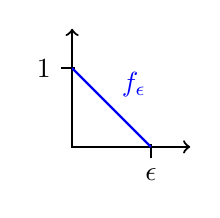
\begin{tikzpicture}[thick]
                \draw [<->] (1.5,0) -- (0,0) -- (0,1.5);
                \draw (1pt,1) -- (-4pt,1) node [left] {$1$};
                \draw (\eps, 1pt) -- (\eps, -4pt) node [below] {$\epsilon$};
                \draw [color=blue] 
                    (0,1) -- node [anchor=south west] {$f_\epsilon$} (\eps,0);
            \end{tikzpicture}
        \end{center}
        Es gilt: $\supnorm{f_\epsilon} = 1,\; \norm{f_\epsilon}_{L^2} \leq
        \sqrt{\epsilon}$.

        Außerdem gilt:
        \begin{align*}
            & \bigl( C^0(\I),\,\supnorm{\,\cdot\,} \bigr)
            \text{ ist Banachraum}
            \\
            & \bigl( C^0(\I),\,\norm{\,\cdot\,}_{L^2} \bigr)
            \text{ ist normierter Vektorraum (aber nicht vollständig)}
        \end{align*}
        Funktionalanalysis lässt sich sinnvoll nur in vollständigen Räumen
        entwickeln. Deshalb werden wir nicht vollständige Räume
        vervollständigen (siehe \cref{vl04:2.18:Vervollstaendigung}).
    \end{enumerate}
\end{thEmpty}


\chapter{Grundstrukturen der Funktionalanalysis}
\begin{thEmpty}[Topologie]
    Sei $X$ eine Menge, $\Topo$ ein System von Teilmengen. Dann heißt $\Topo$
    \emph{Topologie (auf $X$)}, falls gilt:
    \begin{enumerate}[({T}1),labelsep=1em,leftmargin=2cm]
        \item
            \quad $\emptyset\in\Topo,\;X\in\Topo$
        \item
            \quad $\Topo'\subset\Topo \implies \bigcup \Topo' \in \Topo$
        \item
            \quad $T_1,T_2\in\Topo \implies T_1\cap T_2\in\Topo$
    \end{enumerate}

    Ein topologischer Raum $(X,\Topo)$ heißt \emph{Hausdorff-Raum}, falls er
    zusätzlich das Hausdorffsche Trennungsaxiom erfüllt:
    \begin{enumerate}[({T}4),labelsep=1em,leftmargin=2cm]
        \item
            \quad $\forall\, x_1,x_2\in X, x_1\neq x_2\;\; \exists\,
            U_1,U_2\in\Topo\colon\; U_1\cap U_2=\emptyset \wedge x_i\in U_i$
    \end{enumerate}

    Mengen in $\Topo$ heißen \emph{offene Mengen}. Komplemente offener Mengen heißen
    \emph{abgeschlossene Mengen}.

    Eine Menge $W\subset X$ mit $x\in W$ für die eine offene Menge $U$ mit $x\in U$
    und $U\subset W$ existiert, heißt \emph{Umgebung von $x$}.

    Seien $(X,\Topo_X)$ und $(Y,\Topo_Y)$ topologische Räume, so heißt 
    \emph{$f\colon X\to Y$ stetig}, falls die Urbilder offener Mengen stets offen sind.
    (Formal: $\forall\,U'\in\Topo_Y\colon\; f^{-1}(U')\in\Topo_X$)

    Eine Abbildung $f\colon X\to Y$ heißt \emph{stetig in $x\in X$}, falls
    \[ f(x)\in V\in\Topo_Y \qimpliesq \exists\,U\in\Topo_X\colon\; x\in U\subset
        f^{-1}(V)
    \]
    (d.\,h. $f^{-1}(V)$ ist Umgebung von $x$).
\end{thEmpty}

\begin{thEmpty}
    Ist $X$ ein $\K$-Vektorraum mit $\K=\R$ oder $\K=\C$, so heißt $(X,\Topo)$
    \emph{topologischer Vektorraum}, falls $(X,\Topo)$ ein topologischer Raum
    ist und die Abbildungen
    \begin{align*}
        X\times X  &\to X, \quad (x,y)\mapsto x+y \\
        \K\times X &\to X, \quad (\alpha,x)\mapsto \alpha \, x
    \end{align*}
    stetig sind. (\enquote{Algebraische und topologische Struktur sind
    verträglich})
\end{thEmpty}

\begin{thEmpty}[Metrik]
    Ein Tupel $(X,d)$ heißt \emph{metrischer Raum}, falls $X$ eine Menge ist 
    und $d\colon X\times X\to\R$ folgende Bedingungen für alle $x,y,z\in X$ erfüllt:
    \begin{enumerate}[({M}1),labelsep=1em,leftmargin=2cm]
        \item
            $d(x,y)\geq 0 \qundq d(x,y) = 0 \iff x=y$
        \item
            $d(x,y) = d(y,x)$
        \item
            $d(x,z)\leq d(x,y)+d(y,z)$
    \end{enumerate}
    
    Konvergenz:\\
    $\nSeq x$ heißt Cauchy-Folge, falls:
    \[ d(x_k,x_\ell) \to 0 \quad\text{für } k,\ell\to\infty \]
    $x$ heißt Grenzwert von $\nSeq x$ (Notation:
    $x=\lim_{n\to\infty} x_n$ oder: $x_n\to x$ für $n\to\infty$), falls:
    \[ d(x_n,x)\to 0 \quad\text{für } n\to\infty \]
    $(X,d)$ heißt \emph{vollständig}, falls jede Cauchy-Folge einen Grenzwert in
    $X$ besitzt.
    
    Abstand von Mengen $A,B\subset X$:
    \[ \dist(A,B) \defeq \inf \{ d(a,b) \Mid a\in A,\; b\in B \} \]
    Für $A\subset X$ und $x\in X$ definieren wir: $\dist(x,A) \defeq
    \dist(\{x\},A)$.
    
    Für $r\in\R[>0]$ sowie $A\subset X,\;x\in X$ definieren wir:
    \begin{align*}
        & B_r(A) \defeq \{ x\in X \Mid \dist(x,A) < r \}    \\
        & B_r(x) \defeq B_r(\{x\})                          \\
        & \diam(A) \defeq \sup \{ d(a_1,a_2) \Mid a_1,a_2\in A \}
    \end{align*}
    Wir sagen $A$ ist \emph{beschränkt}, falls $\diam(A)<\infty$.
\end{thEmpty}

\begin{thEmpty}[Topologie von Metriken]\label{vl01:topometrik}
    Sei $(X,d)$ ein metrischer Raum und $A\subset X$.
    \begin{align*}
        \setinterior A \defeq \{ x\in X \Mid \exists\,r\in\R[>0]\colon\;
        B_r(x) \subset A \}
        \quad\text{ist das \emph{Innere von $A$}}.
        \\[2ex]
        \setclosure A \defeq \{ x\in X \Mid \forall\,r\in\R[>0]\colon\;
        B_r(x) \cap A \neq \emptyset \}
        \quad\text{ist der \emph{Abschluss von $A$}}.
        \\[2ex]
        \setboundary A \defeq \setclosure A \setminus \setinterior A
        \quad\text{ist der \emph{Rand von $A$}}.
    \end{align*}
    
    Wir sagen, dass $A$ offen ist, falls $\setinterior A = A$ gilt,
    und dass $A$ abgeschlossen ist, falls $\setclosure A = A$ gilt.
    
    Durch die Definition $\Topo \defeq \{ A\subset X \Mid A\text{ offen} \}$
    wird $(X,\Topo)$ zu einem hausdorffschen topologischen Raum.
\end{thEmpty}
